\documentclass[12pt]{article}
\usepackage[margin=1in]{geometry}
\usepackage[T1]{fontenc}
\usepackage[utf8]{inputenc}
\usepackage{lmodern}
\usepackage{microtype}
\usepackage{amsmath,amssymb}
\usepackage{graphicx}
\usepackage{booktabs}
\usepackage{array}
\usepackage{tabularx}
\usepackage{xcolor}
\usepackage{url}
\usepackage[numbers,sort&compress]{natbib}
\usepackage[hidelinks]{hyperref}
\setlength{\emergencystretch}{3em}
\setlength{\Urlmuskip}{0mu plus 1mu}
\newcommand{\care}{\textsc{CARE-State}}
\newcommand{\codeavailability}[1]{\par\medskip\noindent\textbf{Code Availability Statement.} #1\par}
\newcommand{\authorcontributions}[1]{\par\medskip\noindent\textbf{Author Contributions.} #1\par}
\newcommand{\funding}[1]{\par\medskip\noindent\textbf{Funding.} #1\par}
\newcommand{\institutionalreview}[1]{\par\medskip\noindent\textbf{Ethics Approval.} #1\par}
\newcommand{\informedconsent}[1]{\par\medskip\noindent\textbf{Informed Consent.} #1\par}
\newcommand{\dataavailability}[1]{\par\medskip\noindent\textbf{Data Availability Statement.} #1\par}
\newcommand{\conflictsofinterest}[1]{\par\medskip\noindent\textbf{Declaration of Conflicting Interests.} #1\par}
\definecolor{careblue}{RGB}{0,114,178}
\definecolor{carecyan}{RGB}{213,94,0}
\definecolor{caregray}{RGB}{110,110,110}
\definecolor{caredark}{RGB}{0,158,115}
\definecolor{carepurple}{RGB}{204,121,167}
\title{CARE-State: A Missingness-Aware, Survey-Transportable Population Risk State for Short-Term Mortality Surveillance}
\author{Zhi Jin$^{1,*}$ \and Hua Sun$^{1}$ \and Quanwei Sheng$^{1}$ \and Shuang Wu$^{2,*}$\\[4pt]
\parbox{0.88\textwidth}{\centering\small
$^{1}$College of Information Engineering, Changsha Medical University, Changsha 410219, Hunan, China\\
$^{2}$The Affiliated Changsha Central Hospital, Hengyang Medical School, University of South China, Changsha 410004, Hunan, China\\
$^{*}$Correspondence: jinzhi1@csmu.edu.cn; 2018051139@usc.edu.cn}}
\date{}

\begin{document}
\maketitle
\begin{abstract}
Population-health analytics built from public surveys must account for heterogeneous health domains and participant-level differences in which evidence is observed. We developed CARE-State, a missingness-aware and survey-transportable population risk state that represents domain evidence jointly with its availability while separating frozen risk ordering from source-specific probability calibration. The model was developed and tuned on NHANES cycles from 2007--2008 through 2013--2014, with NHANES 2015--2016 reserved as a chronological 36-month test. Frozen checks were then conducted on NHANES 2017--2018 and on NHIS 2017 after calibration using NHIS 2016. In the primary test (5710 participants; 186 events), CARE-State achieved a survey-weighted AUROC of 0.8719 (SD 0.0018) and a Brier score of 0.0208 (SD 0.0001), compared with 0.8671 (SD 0.0058) and 0.0207 (SD 0.0003) for weighted gradient boosting. Its risk-stratum event rates were 0.002, 0.011, and 0.104. Under temporal shift, AUROC was 0.8293--0.8324 and the strata remained ordered at 0.0038, 0.0141, and 0.0876. Under source shift, NHIS 2017 AUROC was 0.8468--0.8507, while calibration reduced Brier error across seeds. Domain masking indicated that demographic evidence contributed most to discrimination, whereas renal evidence most affected probability error. CARE-State provides an auditable population-risk representation for survey-cycle surveillance and evidence-acquisition assessment under the tested shifts; it does not establish causality, universal superiority, or clinical deployment benefit.
\end{abstract}
\noindent\textbf{Keywords:} digital health; public health surveillance; mortality prediction; missing data; survey-weighted prediction; risk stratification; transportability

\section{Introduction and Related Work}
Public health surveys provide a distinctive basis for population risk research because they combine demographic information, self-reported conditions, physical measurements, laboratory assays, survey-design variables, and mortality linkage within a common sampling frame. This breadth supports questions that are difficult to answer from a single clinical service or electronic health-record system, but it also creates a prediction setting in which the available evidence is heterogeneous by design. Modern machine-learning studies in healthcare have demonstrated the potential of high-dimensional prediction, while also emphasizing that performance depends on data provenance, outcome definition, and the relationship between the development population and the population in which a score is used \cite{beam_2018_big_data,esteva_2019_guide,rajkomar_2018_ehr}. In survey-based mortality prediction, therefore, the central methodological problem is not simply to maximize discrimination. It is to construct a risk representation whose meaning remains explicit when measurements, response patterns, and survey sources change.

The target itself has several layers. A short-term mortality model should order individuals according to risk, produce probabilities that correspond to the observed event frequency, and separate clinically meaningful risk strata. These properties are related but not interchangeable: a model can preserve ranking while being systematically miscalibrated, or achieve acceptable average calibration while failing to distinguish the highest-risk group. Prediction-model assessment frameworks consequently recommend reporting discrimination, calibration, clinical or population-level separation, and uncertainty together rather than treating AUROC as a sufficient endpoint \cite{steyerberg_2010_prediction,van_calster_2019_calibration}. In addition, the reliability of an external estimate depends on the number of events and the information available in the validation cohort; sample-size guidance makes this a design issue rather than a post hoc statistical footnote \cite{riley_2020_sample_size,riley_2021_external_validation}.

Missingness is a central part of this problem. In a public survey, an absent laboratory value may reflect a planned subsample, nonresponse, assay availability, or a difference in the survey instrument; it does not automatically represent a normal measurement. Conventional complete-case analysis and naive imputation can remove or obscure that distinction, particularly when the probability of observation varies across clinical domains. General missing-data guidance emphasizes that the mechanism, analysis target, and uncertainty introduced by missingness must be considered together \cite{sterne_2009_imputation,little_2012_missing}. Model-based approaches such as GRU-D and SAITS demonstrate how observation patterns can be incorporated into longitudinal representation learning or time-series imputation \cite{che_2018_grud,du_2023_saits}. Their primary objectives, however, are sequence prediction or value reconstruction. They do not by themselves define an auditable, fixed-horizon mortality state that preserves the distinction between observed low-risk evidence and unavailable evidence, nor do they specify how such a state should be calibrated after transport to a different survey source.

Clinical state representations provide a complementary conceptual foundation. Frailty indices and deficit-accumulation models summarize multidimensional health burden into an interpretable state and have established a useful vocabulary for reasoning about heterogeneous vulnerability \cite{searle_2008_frailty,rockwood_2007_frailty}. A predictive risk state is related to this idea but is not equivalent to a validated frailty index: it is learned against a defined outcome horizon, depends on the measurement process, and must be tested for calibration and transport. The unresolved question is how to retain the interpretability of a domain-level health state while representing whether each domain was actually observed. Without that distinction, a model may assign the same semantic meaning to a low laboratory value and to a laboratory value that was never measured.

Transport introduces a second layer of difficulty. Successive survey cycles can differ in sampling composition, measurement protocols, variable availability, and outcome prevalence; an independent survey source can add different coding conventions and a different feature intersection. These changes are instances of distribution shift, but the relevant question is not whether a model is abstractly domain-invariant. It is whether the population-surveillance properties of the output survive a specified shift. Work on in-the-wild distribution shifts and domain generalization shows that average in-domain performance is an unreliable proxy for out-of-domain behavior \cite{koh_2021_wilds,gulrajani_2021_domain_generalization}. Uncertainty studies further show that probability quality can deteriorate under shift even when ranking appears stable \cite{ovadia_2019_uncertainty}. For public-survey risk models, this motivates a frozen evaluation boundary: the representation and ranking should be tested on a later period or source, while any adjustment of the absolute-risk scale should be isolated in a prespecified calibration step.

The reporting and validation literature provides the corresponding methodological safeguards. TRIPOD and PROBAST require explicit descriptions of cohort construction, outcome definition, missing-data handling, validation, and applicability; the recent TRIPOD+AI update extends this expectation to prediction models using machine-learning methods \cite{collins_2015_tripod,wolff_2019_probaST,collins_2024_tripod_ai}. Survey data add another requirement: estimates must respect the sampling design and its weights, because an unweighted analysis can target a different population quantity from the one implied by the survey protocol \cite{lumley_2004_complex_survey}. NHANES and its public-use linked mortality files provide broad measurements and population follow-up, while NHIS offers a distinct source with a different measurement profile; the official survey and linkage documentation therefore determines which transport claims are defensible \cite{nchs_2024_nhanes_mortality}.

Against this background, we formulate \care as a missingness-aware population risk state rather than as a new entry in a model leaderboard. Each clinical domain is encoded jointly with an availability mask; unavailable evidence is prevented from acquiring the semantics of a normal value, and the available domains are combined into a shared state that supports both absolute-risk estimation and ordered risk stratification. The representation is frozen before the temporal and source tests. In the intended digital-health workflow, a survey or registry pipeline can use the state to monitor risk strata across cycles, identify when probability recalibration is required, and prioritize which evidence domains should be collected or audited when measurement capacity is constrained. A separate, prespecified calibration adapter may alter the probability scale for a new source, but it does not retrain the domain encoders or change the frozen ranking. This separation makes it possible to ask two distinct questions: whether the ordering of risk is transported, and whether the absolute probabilities require source-specific recalibration.

The present study makes four connected contributions. First, it gives an auditable formulation of a domain-gated risk state in which population-health evidence and evidence availability are modeled as different objects. Second, it evaluates the state on a prespecified later NHANES cycle and reports discrimination, calibration, and ordered risk-stratum event rates together. Third, it performs an independent NHIS survey-source transport test using a reduced, prespecified feature intersection and validation-only calibration. Fourth, it uses controlled domain masking to identify whether each clinical domain primarily affects discrimination or probability accuracy. The resulting evidence is intended to define the operating boundary of a population risk state under the tested survey shifts, not to establish causality, universal superiority, or clinical deployment benefit.

\section{Materials and Methods}
\subsection{Data sources and analytic design}
The analysis uses public-use NHANES cycles linked to publicly released mortality follow-up files and an independent NHIS survey-source transport test. The survey and linkage resources are maintained by the National Center for Health Statistics \cite{nchs_2024_nhanes_mortality}. The outcome is all-cause death within the analysis-specific horizon; participants without sufficient public-use follow-up for that horizon were not included in the corresponding evaluation block. The data sources provide survey measurements, design variables, and fixed-horizon mortality outcomes without introducing a new participant contact or intervention. The feature map is organized into four clinical domains: demographic, metabolic, cardiovascular, and renal. The domains are kept separate throughout the analysis so that their evidence availability, contribution to the shared state, and response to domain masking can be examined independently.

The chronological design separates model development, temporal evaluation, source-specific calibration, and independent-source testing. NHANES cycles from 2007--2008 through 2013--2014 define the development and validation pool; NHANES 2015--2016 is excluded from fitting and tuning and reserved as the primary 36-month temporal test. The 2013--2014 validation cycle supplies the validation-only calibration parameters used for the primary NHANES calibration audit and the later temporal check. NHANES 2017--2018 is evaluated only after model freezing as a later 24-month temporal check. NHIS 2016 is used only to estimate the source-specific calibration adapter, and NHIS 2017 is held out for the final independent survey-source transport test. For NHIS, the input is restricted to the prespecified self-report/BMI feature intersection shared with NHANES. This design allows the external analysis to test transport of the learned state and calibration procedure without retraining the representation on the target test cohort.

The complete data-to-evaluation framework is summarized in Figure~\ref{fig:framework}. It links the public survey evidence, domain-gated representation, shared clinical risk state, ordered risk interpretation, and the frozen temporal and cross-source validation boundaries.

\begin{figure}[t!]
\centering
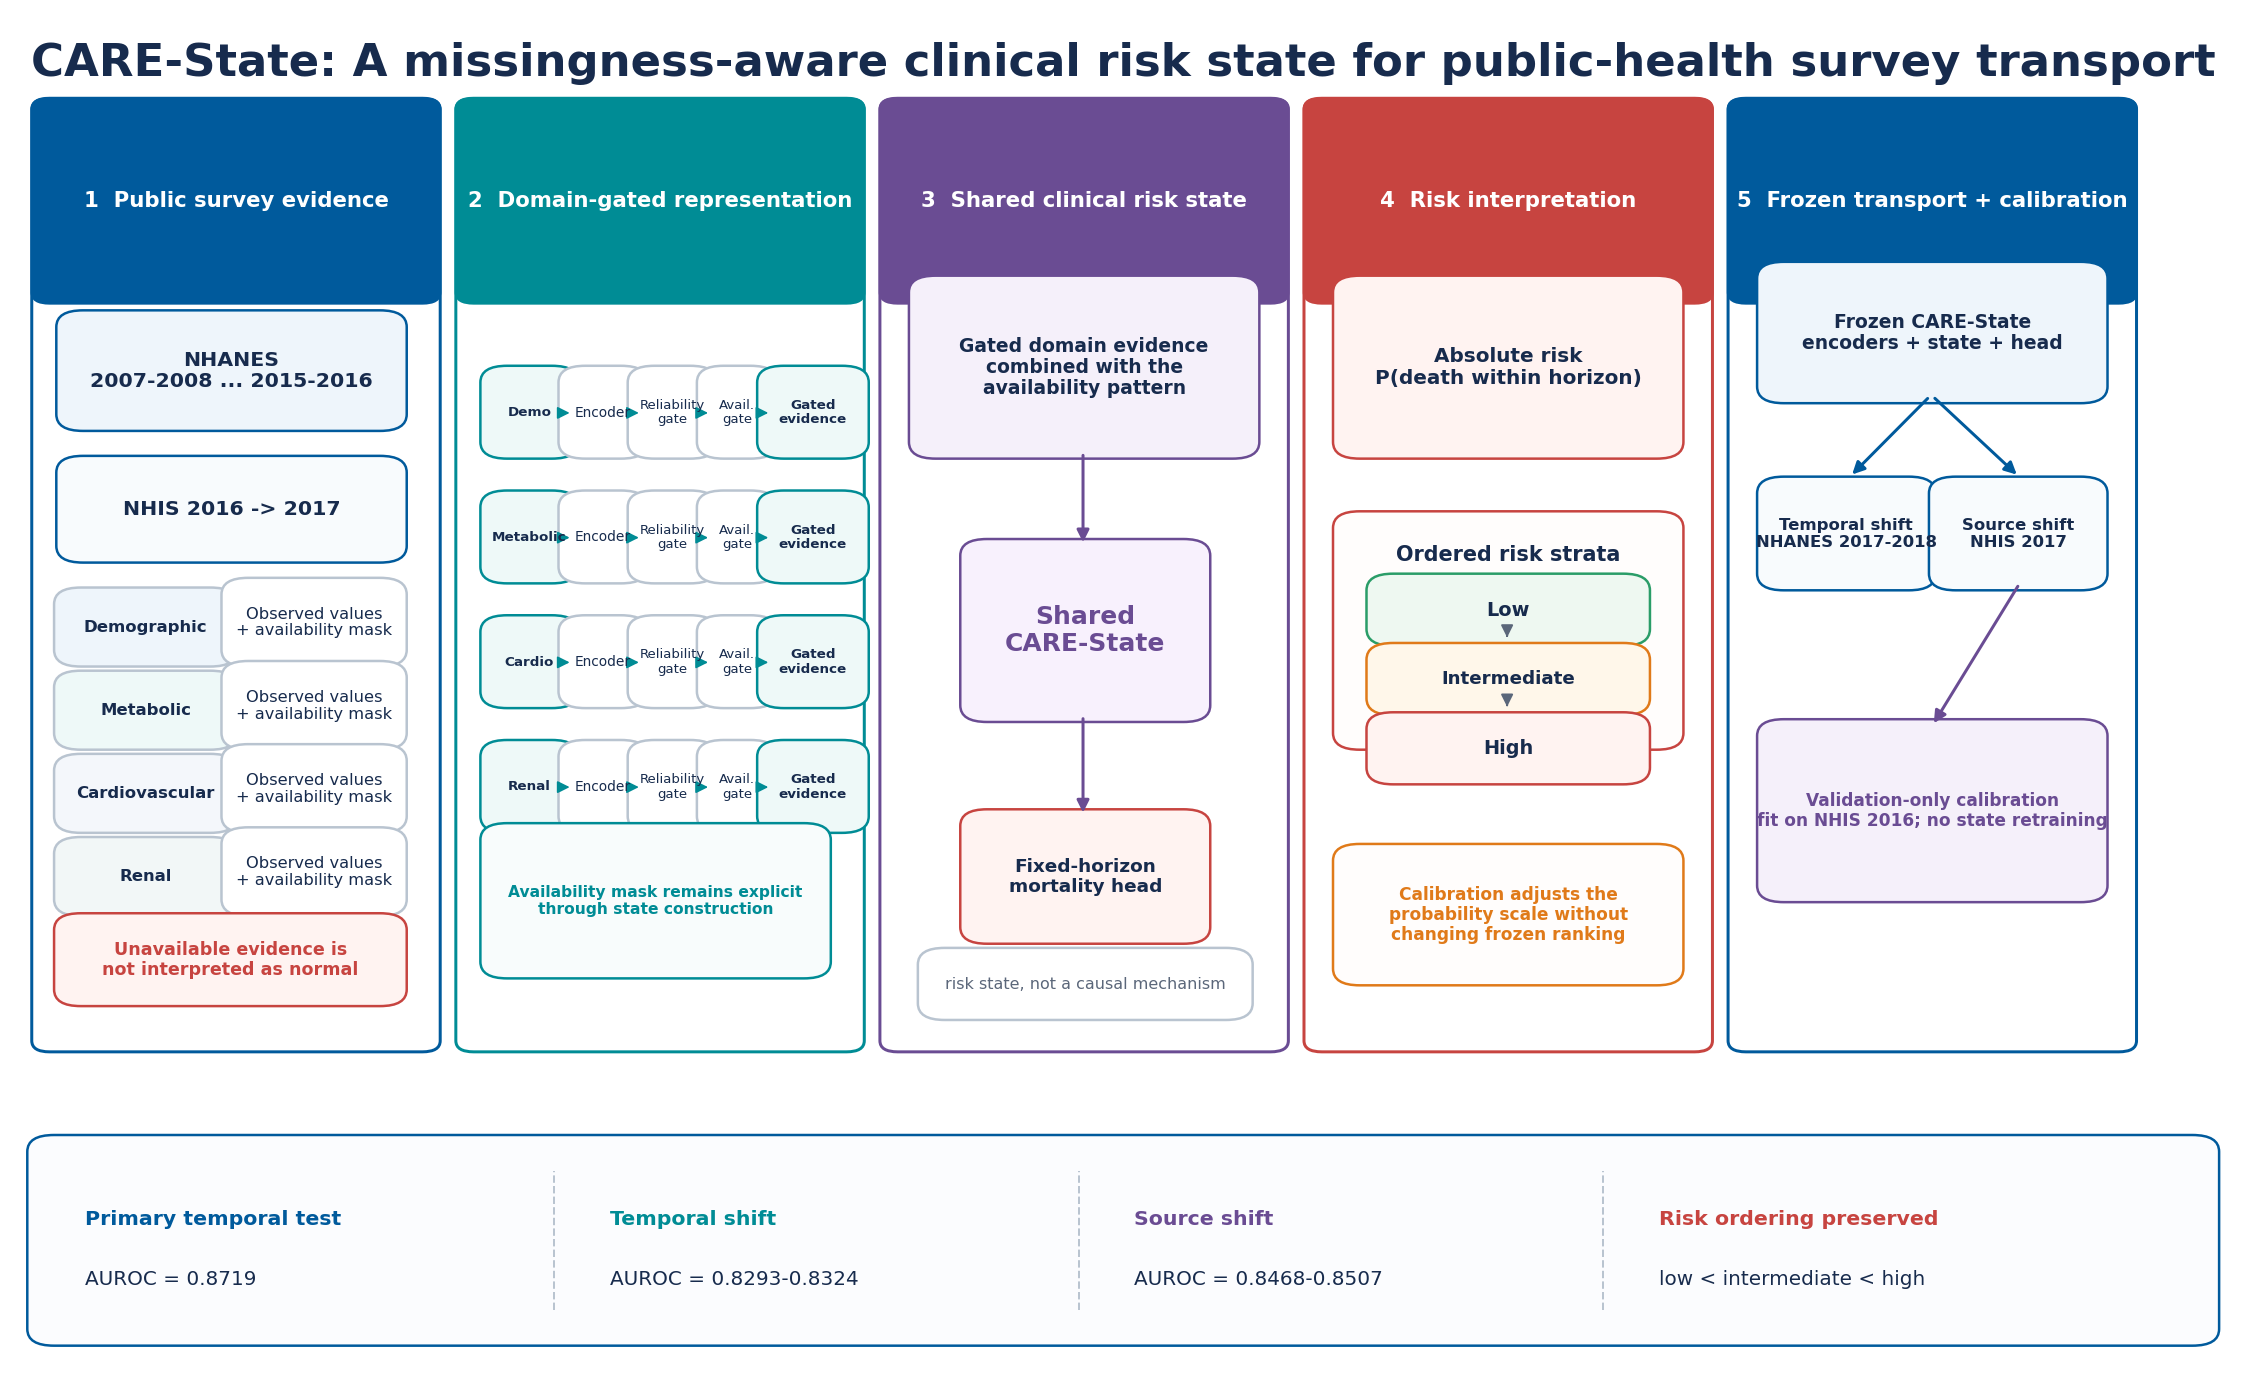
\includegraphics[width=\linewidth]{care_state_framework_en.png}
\caption{CARE-State framework from public survey evidence to domain-gated representation, shared clinical risk state, risk interpretation, and frozen transport with validation-only calibration.}
\label{fig:framework}
\end{figure}

\subsection{Problem Definition}
Let $\mathcal{D}=\{\mathrm{demographic},\mathrm{metabolic},\mathrm{cardiovascular},\mathrm{renal}\}$ denote the clinical domains. For participant $i$, $x_i^{(d)}$ is the measurement vector in domain $d$, $m_i^{(d)}\in\{0,1\}$ records whether that domain is available after the prespecified data audit, and $m_i=(m_i^{(d)}:d\in\mathcal{D})$ is the complete availability vector. The mask is determined from data availability and is not generated from the mortality outcome. Let $Y_i(h)$ denote the indicator of death within the analysis-specific horizon $h$. The target conditional risk is
\begin{equation}
 p_i(h)=P\left(Y_i(h)=1\mid x_i,m_i\right),
 \label{eq:target-risk}
\end{equation}
with the model output $\hat p_i(h)$ estimating $p_i(h)$. The primary temporal analysis uses $h=36$ months. The NHANES 2017--2018 and NHIS analyses use $h=24$ months because the available public mortality linkage does not provide equivalent 36-month coverage for all participants in those analysis blocks. Participants were filtered before metric calculation so that the event indicator represented the same fixed horizon within each block.

The formulation distinguishes three objects that are often conflated in a missing-data prediction pipeline: the measured value $x_i^{(d)}$, the fact that the domain is available $m_i^{(d)}$, and the resulting risk estimate $\hat p_i(h)$. A domain with $m_i^{(d)}=0$ is therefore not interpreted as a normal or low-risk measurement. Its contribution is removed by the domain gate, while the mask remains available to the state function. This distinction is central to the study question because the analysis evaluates whether the risk state remains ordered when the composition of available evidence changes.

The model-fitting boundary is defined before the frozen temporal and source tests. The 2015--2016 NHANES cycle is not used for representation fitting, hyperparameter selection, early stopping, threshold selection, or calibration; NHANES 2017--2018 and NHIS 2017 are evaluated only after the model is frozen. For the primary NHANES calibration audit and the later temporal check, calibration parameters were estimated only on the 2013--2014 validation cycle. For the independent source test, calibration parameters were estimated only on NHIS 2016. These adapters are not used to change the domain encoders, shared state, or ranking induced by the frozen model.

\subsection{CARE-State representation}
\care encodes each clinical domain separately before combining the available evidence. For domain $d$, an encoder maps the domain measurements to $z_i^{(d)}=f_d(x_i^{(d)})$. A reliability gate produces an evidence-quality coefficient from the domain measurements and availability mask and then applies the hard availability gate:
\begin{equation}
 \tilde z_i^{(d)}=m_i^{(d)}g_i^{(d)}z_i^{(d)},\qquad
 g_i^{(d)}=\sigma\left(a_d(x_i^{(d)},m_i^{(d)})\right).
 \label{eq:domain-gate}
\end{equation}
Because $m_i^{(d)}$ multiplies the complete domain representation, an unavailable domain contributes exactly zero to the aggregated evidence in Equation~\ref{eq:domain-gate}; its measurement vector cannot be reinterpreted as observed solely because a preprocessing value exists. The shared state is then formed from the gated domain evidence and the full availability pattern:
\begin{equation}
 s_i=\phi\left(\sum_{d\in\mathcal{D}}\tilde z_i^{(d)},m_i\right),
 \label{eq:shared-state}
\end{equation}
and the mortality head produces
\begin{equation}
 \hat p_i(h)=\sigma\left(q_h(s_i)\right).
 \label{eq:risk-head}
\end{equation}
Equations~\ref{eq:domain-gate}--\ref{eq:risk-head} define the information path used in all reported evaluations: domain-specific evidence is first filtered by availability and reliability, the filtered evidence is combined into a state, and the state is mapped to a fixed-horizon risk. The state is therefore a representation of available clinical evidence, rather than a claim that the missingness pattern itself is a causal clinical signal.

The clinical gate is used to constrain the interpretation of the state, not to assert that every clinical variable has a universally monotonic effect. For the audited variables with a prespecified directional sign $\delta_j\in\{-1,+1\}$, the directional constraint can be written as
\begin{equation}
 \delta_j\frac{\partial q_h(s_i)}{\partial x_{ij}}\geq 0,
 \qquad j\in\mathcal{J}_{\mathrm{constrained}},
 \label{eq:directional-constraint}
\end{equation}
where $\mathcal{J}_{\mathrm{constrained}}$ contains only variables for which the audited feature definition supports an ordered interpretation. Variables with ambiguous direction are excluded from Equation~\ref{eq:directional-constraint}. The constraint is consequently a structural interpretability condition on the risk state; it is not evidence of a biological mechanism or a guarantee that the constrained representation improves AUROC.

Three independent random seeds were used for the closeout experiment, with the same early-stopping protocol and evaluation boundary for every seed. The aggregate manuscript package retains the resulting seed-level metrics and figure-generation inputs; individual-level records and the original server-side training pipeline are not included in the submission archive. The equations above specify the information path and evaluation boundary, while the repository documents the aggregate-result and figure-reproduction layer. Consequently, the present study makes a bounded claim about the evaluated risk-state behavior rather than claiming that the submission archive alone is a complete retraining environment.

The compact information path used for inference and evaluation is shown in Figure~\ref{fig:workflow}; the larger framework in Figure~\ref{fig:framework} places this path within the survey, transport, and calibration design.

\begin{figure}[t!]
\centering
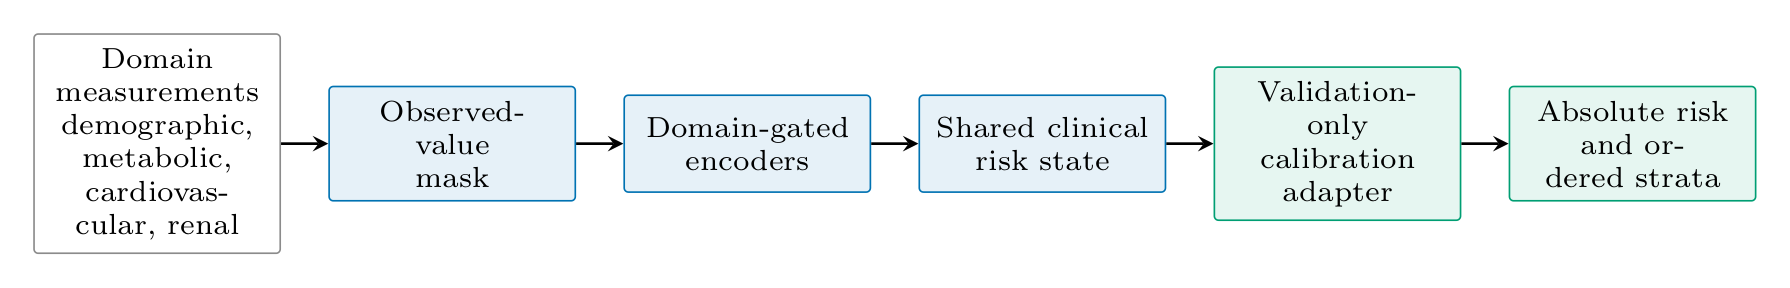
\includegraphics[width=\linewidth]{workflow.png}
\caption{CARE-State processing and evaluation boundary. Each clinical domain is represented together with an observed-value mask before the shared risk state is formed. The frozen state is transported to a new survey source; only the prespecified calibration adapter may be fitted on a separate calibration cohort.}
\label{fig:workflow}
\end{figure}

\subsection{Cohort-specific calibration}
When the frozen state is transported to a new survey source, a two-parameter calibration adapter is fitted on a separate calibration cohort. The adapter operates on the frozen probability and is expressed in logit form as
\begin{equation}
 \operatorname{logit}(\tilde p_i)=\alpha+\beta\operatorname{logit}(\hat p_i).
 \label{eq:calibration-adapter}
\end{equation}
The derivative of the inverse-logit transformation is
\begin{equation}
 \frac{\partial \tilde p_i}{\partial \hat p_i}
 =\frac{\beta\,\tilde p_i(1-\tilde p_i)}{\hat p_i(1-\hat p_i)}.
 \label{eq:calibration-derivative}
\end{equation}
Thus, when the fitted adapter has $\beta>0$, it preserves the ordering induced by the frozen model while changing the intercept and slope of the absolute-risk scale. Equations~\ref{eq:calibration-adapter} and~\ref{eq:calibration-derivative} formalize the separation used in this study: transport of relative risk is assessed from the frozen state, whereas calibration is estimated using only the prespecified calibration cohort. The adapter does not retrain the domain encoders, shared state, or mortality head. Raw and adapted results are reported separately whenever both are available.

\subsection{Training and evaluation protocol}
The closeout experiment used three independent random seeds and the same early-stopping protocol for each seed. Each seed produced a separate fitted model; the reported mean and standard deviation describe variation across these training realizations. No target-test outcome was used to select a seed, retrain the representation, or fit a transport adapter. The weighted Cox model and weighted gradient-boosting model used the same audited feature map, cohort boundary, survey-design weights, and prediction horizon as the CARE-State comparison. The Cox model follows the proportional-hazards formulation \cite{cox_1972_regression}; tree-based comparators are contextualized by XGBoost, LightGBM, and CatBoost \cite{chen_2016_xgboost,ke_2017_lightgbm,prokhorenkova_2018_catboost}.

Let $w_i$ denote the survey-design weight and $\mathcal{I}$ the participants in an evaluation cohort. The weighted Brier score was computed as
\begin{equation}
 \operatorname{Brier}_w(h)=
 \frac{\sum_{i\in\mathcal{I}}w_i\left(Y_i(h)-\hat p_i(h)\right)^2}
 {\sum_{i\in\mathcal{I}}w_i}.
 \label{eq:weighted-brier}
\end{equation}
For a prespecified risk stratum $G_k$, the corresponding weighted event rate was
\begin{equation}
 \hat e_{k,w}(h)=
 \frac{\sum_{i\in\mathcal{I}}w_iY_i(h)\,\mathbb{1}\{i\in G_k\}}
 {\sum_{i\in\mathcal{I}}w_i\,\mathbb{1}\{i\in G_k\}}.
 \label{eq:weighted-stratum-rate}
\end{equation}
The primary discrimination measure was survey-weighted AUROC. For positive participants $i$ and negative participants $j$, it was calculated as
\begin{equation}
 \operatorname{AUROC}_w=\frac{\sum_{i:Y_i=1}\sum_{j:Y_j=0}w_iw_j\left[\mathbb{1}(\hat p_i>\hat p_j)+\frac{1}{2}\mathbb{1}(\hat p_i=\hat p_j)\right]}{\left(\sum_{i:Y_i=1}w_i\right)\left(\sum_{j:Y_j=0}w_j\right)}.
 \label{eq:weighted-auroc}
\end{equation}
The same survey-design weights were used in the positive and negative contributions. Equations~\ref{eq:weighted-brier}--\ref{eq:weighted-auroc} and~\ref{eq:weighted-stratum-rate} make explicit why discrimination and risk-stratum analyses are reported together: AUROC evaluates ordering, whereas the weighted Brier score and stratum event rates evaluate probability error and population-level separation.

Calibration was assessed by ordering participants according to the frozen prediction, dividing the primary test cohort into ten prediction deciles, and comparing weighted mean predicted risk with the weighted observed event rate in each decile. For the primary NHANES calibration audit and the later temporal check, the two-parameter adapter was fitted on NHANES 2013--2014 only; for the NHIS source test, it was fitted on NHIS 2016 only. Neither adapter used outcomes from its corresponding test cohort. For transport comparisons, paired participant bootstrap resampling was used to recompute the metric difference. For bootstrap replicate $b$, the contrast was defined as
\begin{equation}
 \Delta^{(b)}=M^{(b)}_{w,\mathrm{CARE}}-M^{(b)}_{w,\mathrm{reference}},
 \label{eq:bootstrap-contrast}
\end{equation}
and the reported interval was obtained from the empirical bootstrap distribution of $\Delta^{(b)}$. This paired construction preserves the comparison set within each replicate and separates uncertainty in the contrast from variation across random training seeds.

\subsection{Missingness stress audit}
To characterize the failure boundary of the state when one information domain is unavailable at inference time, we applied a controlled domain-masking audit to the NHANES 2015--2016 test cohort. The three risk strata were assigned with fixed development-phase cutpoints and applied unchanged to every evaluation cohort; no test-cohort outcome or prediction quantile was used to redefine the strata. For domain $d$, the perturbed mask was defined as
\begin{equation}
 m_{i,-d}^{(r)}=\begin{cases}
 0,&r=d,\\
 m_i^{(r)},&r\neq d,
 \end{cases}
 \qquad r\in\mathcal{D},
 \label{eq:masking-perturbation}
\end{equation}
while the remaining domain measurements and the fitted model parameters were held fixed. The perturbed prediction $\hat p_{i,-d}(h)$ was then evaluated with the same weighted metrics as the complete-input prediction. The change in each metric was reported as
\begin{equation}
 \Delta M_{-d}=M\left(\hat p_{-d}\right)-M\left(\hat p_{\mathrm{complete}}\right).
 \label{eq:masking-change}
\end{equation}
Equations~\ref{eq:masking-perturbation} and~\ref{eq:masking-change} define a controlled sensitivity analysis: they identify which performance dimension deteriorates when a domain is removed from inference, without retraining the model or treating the perturbation as a beneficial form of missingness. The audit does not reproduce every mechanism of nonresponse in a real survey and is interpreted as a failure-mode analysis rather than a causal missingness experiment.

\section{Results}
\subsection{Cohort composition and evidence availability}
The cohorts were organized to answer separate questions about discrimination, temporal stability, source transport, and evidence dependence. The five NHANES cycles from 2007--2008 through 2015--2016 contributed 29,571 eligible participants and 3,135 all-cause events, with the first four cycles used for model development and validation. NHANES 2015--2016 was excluded from fitting and tuning and reserved as the primary 36-month temporal test; it contained 5,710 participants with 186 events. The later NHANES 2017--2018 cycle provided a second frozen evaluation at 24 months, with 2,910 participants and 110 events. For the independent survey-source transport analysis, NHIS 2016 supplied the calibration cohort (32,487 participants and 797 events), whereas NHIS 2017 was held out as the final test cohort (26,267 participants and 656 events). The NHIS analysis used the prespecified self-report/BMI feature intersection shared with NHANES, so that transport assessed the frozen state and calibration adapter rather than a newly optimized representation.

This sequence establishes an ordered evidence chain. The primary NHANES analysis asks whether the model can rank risk after a time-separated split; the later NHANES cycle tests whether that ordering persists under an additional period shift; and the NHIS block changes both the survey source and the measurement composition. The prediction horizons were kept distinct because the public linkage files do not provide equivalent follow-up coverage: the primary NHANES test uses 36 months, while the later NHANES and NHIS transport checks use 24 months. Consequently, the transport results are interpreted as stability of the risk state under the specified horizon and cohort changes, rather than as direct numerical replications of the primary test. Participant counts, event counts, horizons, and analytical roles are summarized in Table~\ref{tab:cohorts}.

The common feature map was highly observed in aggregate, but its observation profile differed systematically by clinical domain. Mean weighted coverage was highest for demographic variables (98.2\%), followed by metabolic (96.8\%), cardiovascular (96.5\%), and renal variables (96.4\%). Across cycles, demographic coverage ranged from 98.0\% to 98.4\%, whereas renal coverage ranged from 95.7\% to 96.9\%; the corresponding metabolic and cardiovascular ranges were 96.4--97.0\% and 95.9--97.4\%, respectively (Figure~\ref{fig:coverage}, Table~\ref{tab:coverage}). The aggregate rates therefore do not describe a completely uniform input: the renal domain was consistently the least observed, and cardiovascular coverage showed the widest cycle-to-cycle range. This pattern provides the empirical basis for carrying an availability mask with the domain measurements. CARE-State was evaluated in a setting where most variables were present, but where the availability of clinically distinct evidence was not interchangeable across domains or survey cycles.

\begin{figure}[t!]
\centering
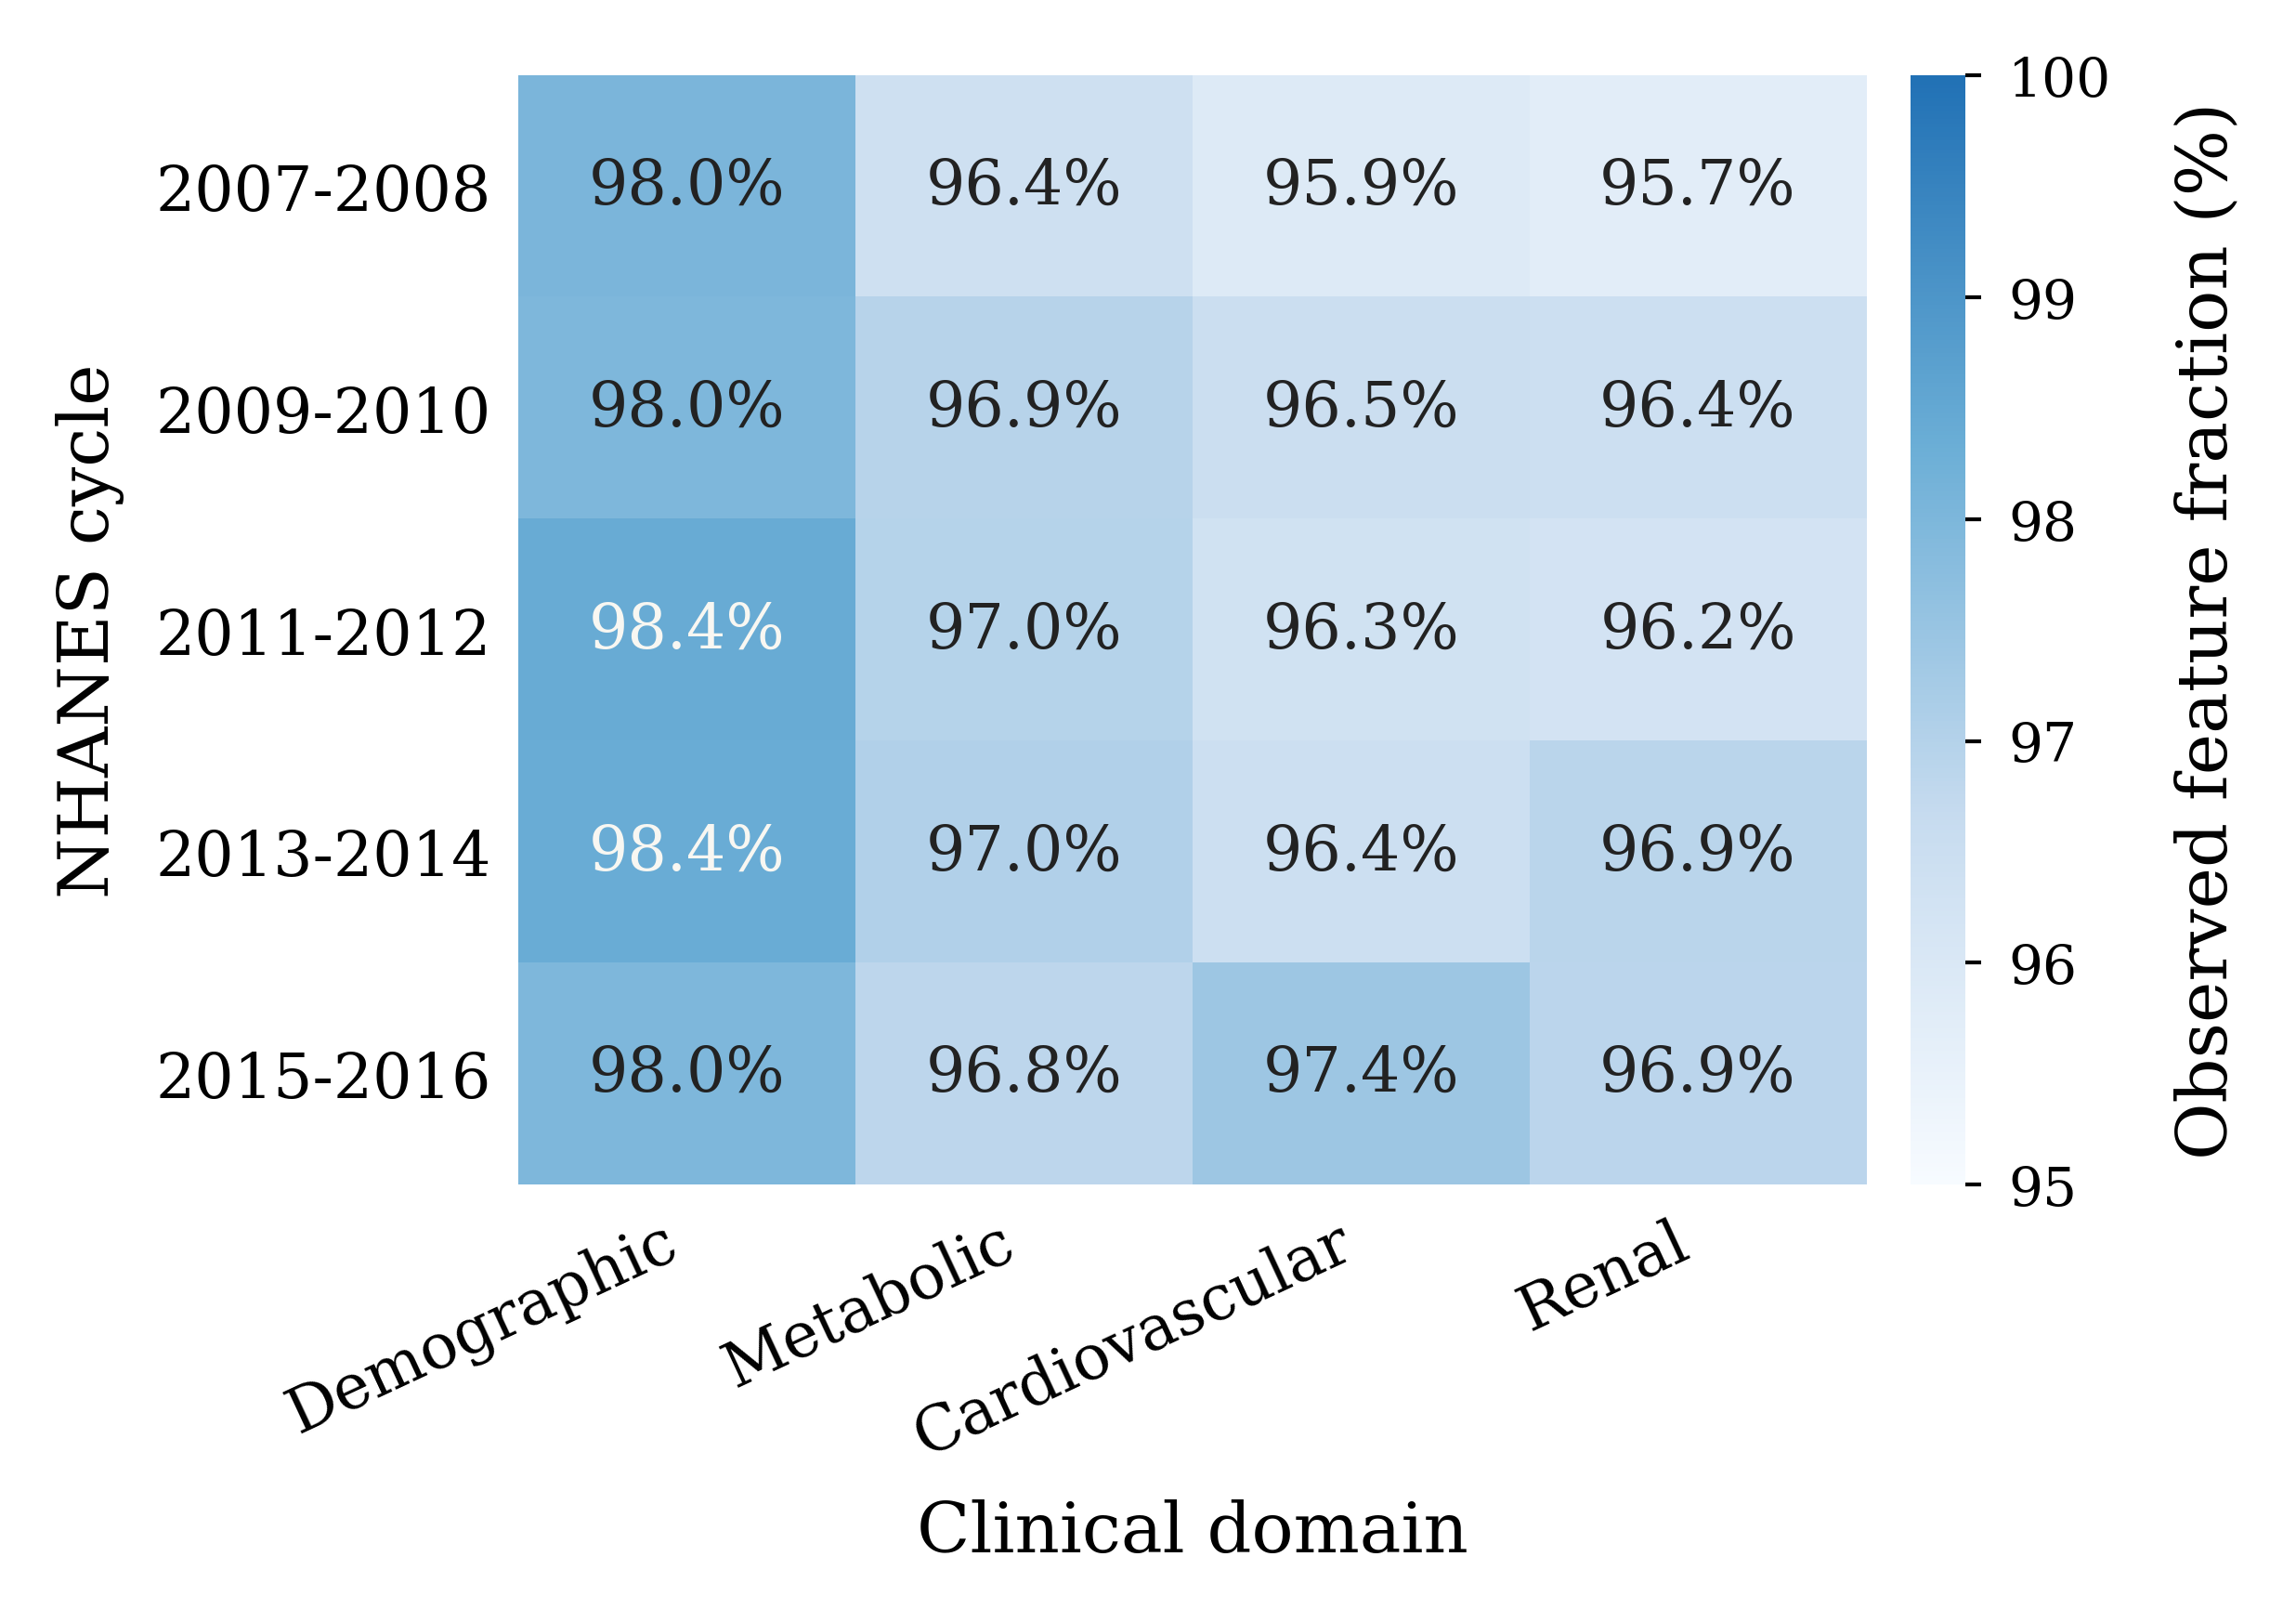
\includegraphics[width=0.78\linewidth]{domain_coverage_heatmap.png}
\caption{Weighted observed-variable coverage across the five NHANES cycles used for development and temporal testing. Each cell reports the weighted fraction of variables observed within a clinical domain.}
\label{fig:coverage}
\end{figure}

\begin{table}[t]
\centering
\caption{Cycle-level weighted observed-variable coverage summary. Values are the mean and range across the five NHANES cycles.}
\label{tab:coverage}
\begin{tabular}{lcc}
\toprule
Clinical domain & Mean coverage (\%) & Range across cycles (\%) \\
\midrule
Demographic & 98.2 & 98.0--98.4 \\
Metabolic & 96.8 & 96.4--97.0 \\
Cardiovascular & 96.5 & 95.9--97.4 \\
Renal & 96.4 & 95.7--96.9 \\
\bottomrule
\end{tabular}
\end{table}

\begin{table}[t]
\centering
\caption{Cohort composition and analytical roles.}
\label{tab:cohorts}
\begin{tabular}{p{0.42\linewidth}rrp{0.22\linewidth}}
\toprule
Analysis block & Participants & Events & Role \\
\midrule
NHANES 2007--2008 to 2013--2014 & 23,861 & 2,949 & Model development and validation \\
NHANES 2015--2016, 36 months & 5,710 & 186 & Primary temporal test \\
NHANES 2017--2018, 24 months & 2,910 & 110 & Frozen temporal check \\
NHIS 2016, 24 months & 32,487 & 797 & Calibration cohort \\
NHIS 2017, 24 months & 26,267 & 656 & Independent-source test \\
\bottomrule
\end{tabular}
\end{table}

\subsection{Primary temporal discrimination and risk stratification}
On the NHANES 2015--2016 36-month test, \care achieved a weighted AUROC of 0.8719 (SD 0.0018) and a Brier score of 0.0208 (SD 0.0001) across three seeds. The weighted GBM produced an AUROC of 0.8671 (SD 0.0058) and a Brier score of 0.0207 (SD 0.0003), whereas the weighted Cox model produced 0.7857 and 0.0226, respectively. The comparison separates two aspects of performance. CARE-State exceeded GBM by 0.0048 AUROC points and Cox by 0.0862 points, indicating a clear advantage over the proportional-hazards reference and only a small discrimination margin over the nonlinear tree model. In contrast, the Brier scores of CARE-State and GBM differed by just 0.0001, while Cox was 0.0018 higher than CARE-State. Thus, the primary test supports competitive discrimination and probability accuracy, but the two nonlinear models occupy essentially the same calibration-error range. The low three-seed variability of CARE-State, particularly for Brier score, indicates that this pattern was stable across the reported training realizations rather than being attributable to one favorable seed (Figure~\ref{fig:primary}, Table~\ref{tab:primary}).

The structural interpretation of the model is also important for reading this comparison. The aggregate ablation results did not establish an AUROC gain for the complete model over the corresponding no-gate or no-monotonic variants. The domain gate and directional constraints should consequently be evaluated by whether they make evidence availability and risk ordering auditable, not by an unsupported claim that each component necessarily increases discrimination. This distinction is consistent with the primary metrics: the proposed state is a representation and evaluation framework whose value is expressed across ranking, calibration, transport, and failure analysis rather than by a single point estimate.

Risk stratification supplied a second, clinically interpretable axis of performance. CARE-State divided the primary test cohort into low-, intermediate-, and high-risk strata with weighted event rates of approximately 0.002, 0.011, and 0.104. The absolute separation between the low- and high-risk strata was 0.102, and the high-risk event rate was about 52 times the low-risk rate; the intermediate group occupied a distinct level rather than collapsing into either extreme. This result shows that the shared state was not only ordering individual scores, but also producing population groups with materially different observed event frequencies. The stratified analysis therefore complements AUROC, which summarizes pairwise ordering but does not show how the score partitions the population into usable risk levels. Figure~\ref{fig:primary} places the discrimination and probability-error results on common axes, while Table~\ref{tab:primary} preserves the seed-level estimates used for comparison.

\begin{figure}[t!]
\centering
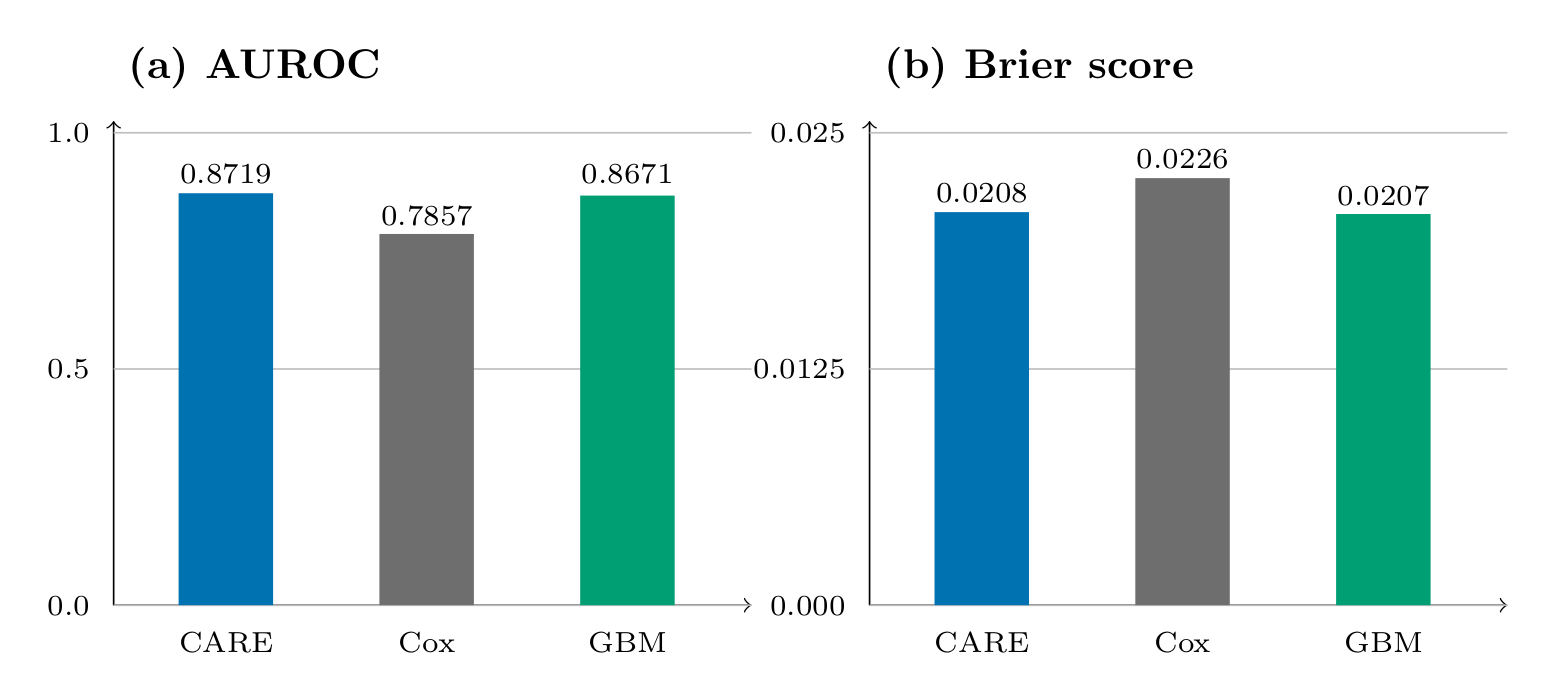
\includegraphics[width=\linewidth]{primary.png}
\caption{Primary 36-month NHANES temporal test. Bars show the reported mean weighted AUROC (a) and Brier score (b) for CARE-State, weighted Cox, and weighted GBM; the numerical values are the same as Table~\ref{tab:primary}.}
\label{fig:primary}
\end{figure}

\begin{table}[t]
\centering
\caption{Primary 36-month NHANES temporal test across three seeds.}
\label{tab:primary}
\begin{tabular}{lcc}
\toprule
Model & Weighted AUROC (mean $\pm$ SD) & Brier score (mean $\pm$ SD) \\
\midrule
CARE-State & 0.8719 $\pm$ 0.0018 & 0.0208 $\pm$ 0.0001 \\
Weighted Cox & 0.7857 $\pm$ 0.0000 & 0.0226 $\pm$ 0.0000 \\
Weighted GBM & 0.8671 $\pm$ 0.0058 & 0.0207 $\pm$ 0.0003 \\
\bottomrule
\end{tabular}
\end{table}

The calibration analysis clarified how the risk state behaved on the absolute-risk scale. Across the ten prediction deciles, the weighted observed event rate increased overall from approximately 0 in the lowest decile to 0.1798 in the highest decile. The pattern was not perfectly monotonic at every adjacent decile: the sixth decile fell to 0.0026 after 0.0105 in the fifth, indicating local sampling variation within an otherwise strong risk gradient. The uncalibrated predictions ranged from 0.0015 to 0.2142. After the validation-only adapter, the prediction range shifted to 0.0023--0.2311, while the observed rates remained fixed because the adapter changes the absolute-risk scale without changing participant ordering.

The adjustment was most informative in the central part of the distribution. The fifth-decile prediction moved from 0.0059 to 0.0082, closer to the observed rate of 0.0105, and the seventh-decile prediction moved from 0.0145 to 0.0191, close to the observed rate of 0.0201. The same transformation did not improve every decile: at the upper end, the tenth-decile estimate increased from 0.2142 to 0.2311 while the observed rate was 0.1798. The calibration evidence therefore describes a structured, partial correction rather than a uniform improvement across the entire probability range. Its main effect was to bring several low-to-intermediate risk estimates toward the observed scale while retaining a clearly separated upper tail. The adapter used for this audit was estimated only on NHANES 2013--2014 and did not use outcomes from the 2015--2016 test (Figure~\ref{fig:calibration}).

\begin{figure}[t!]
\centering
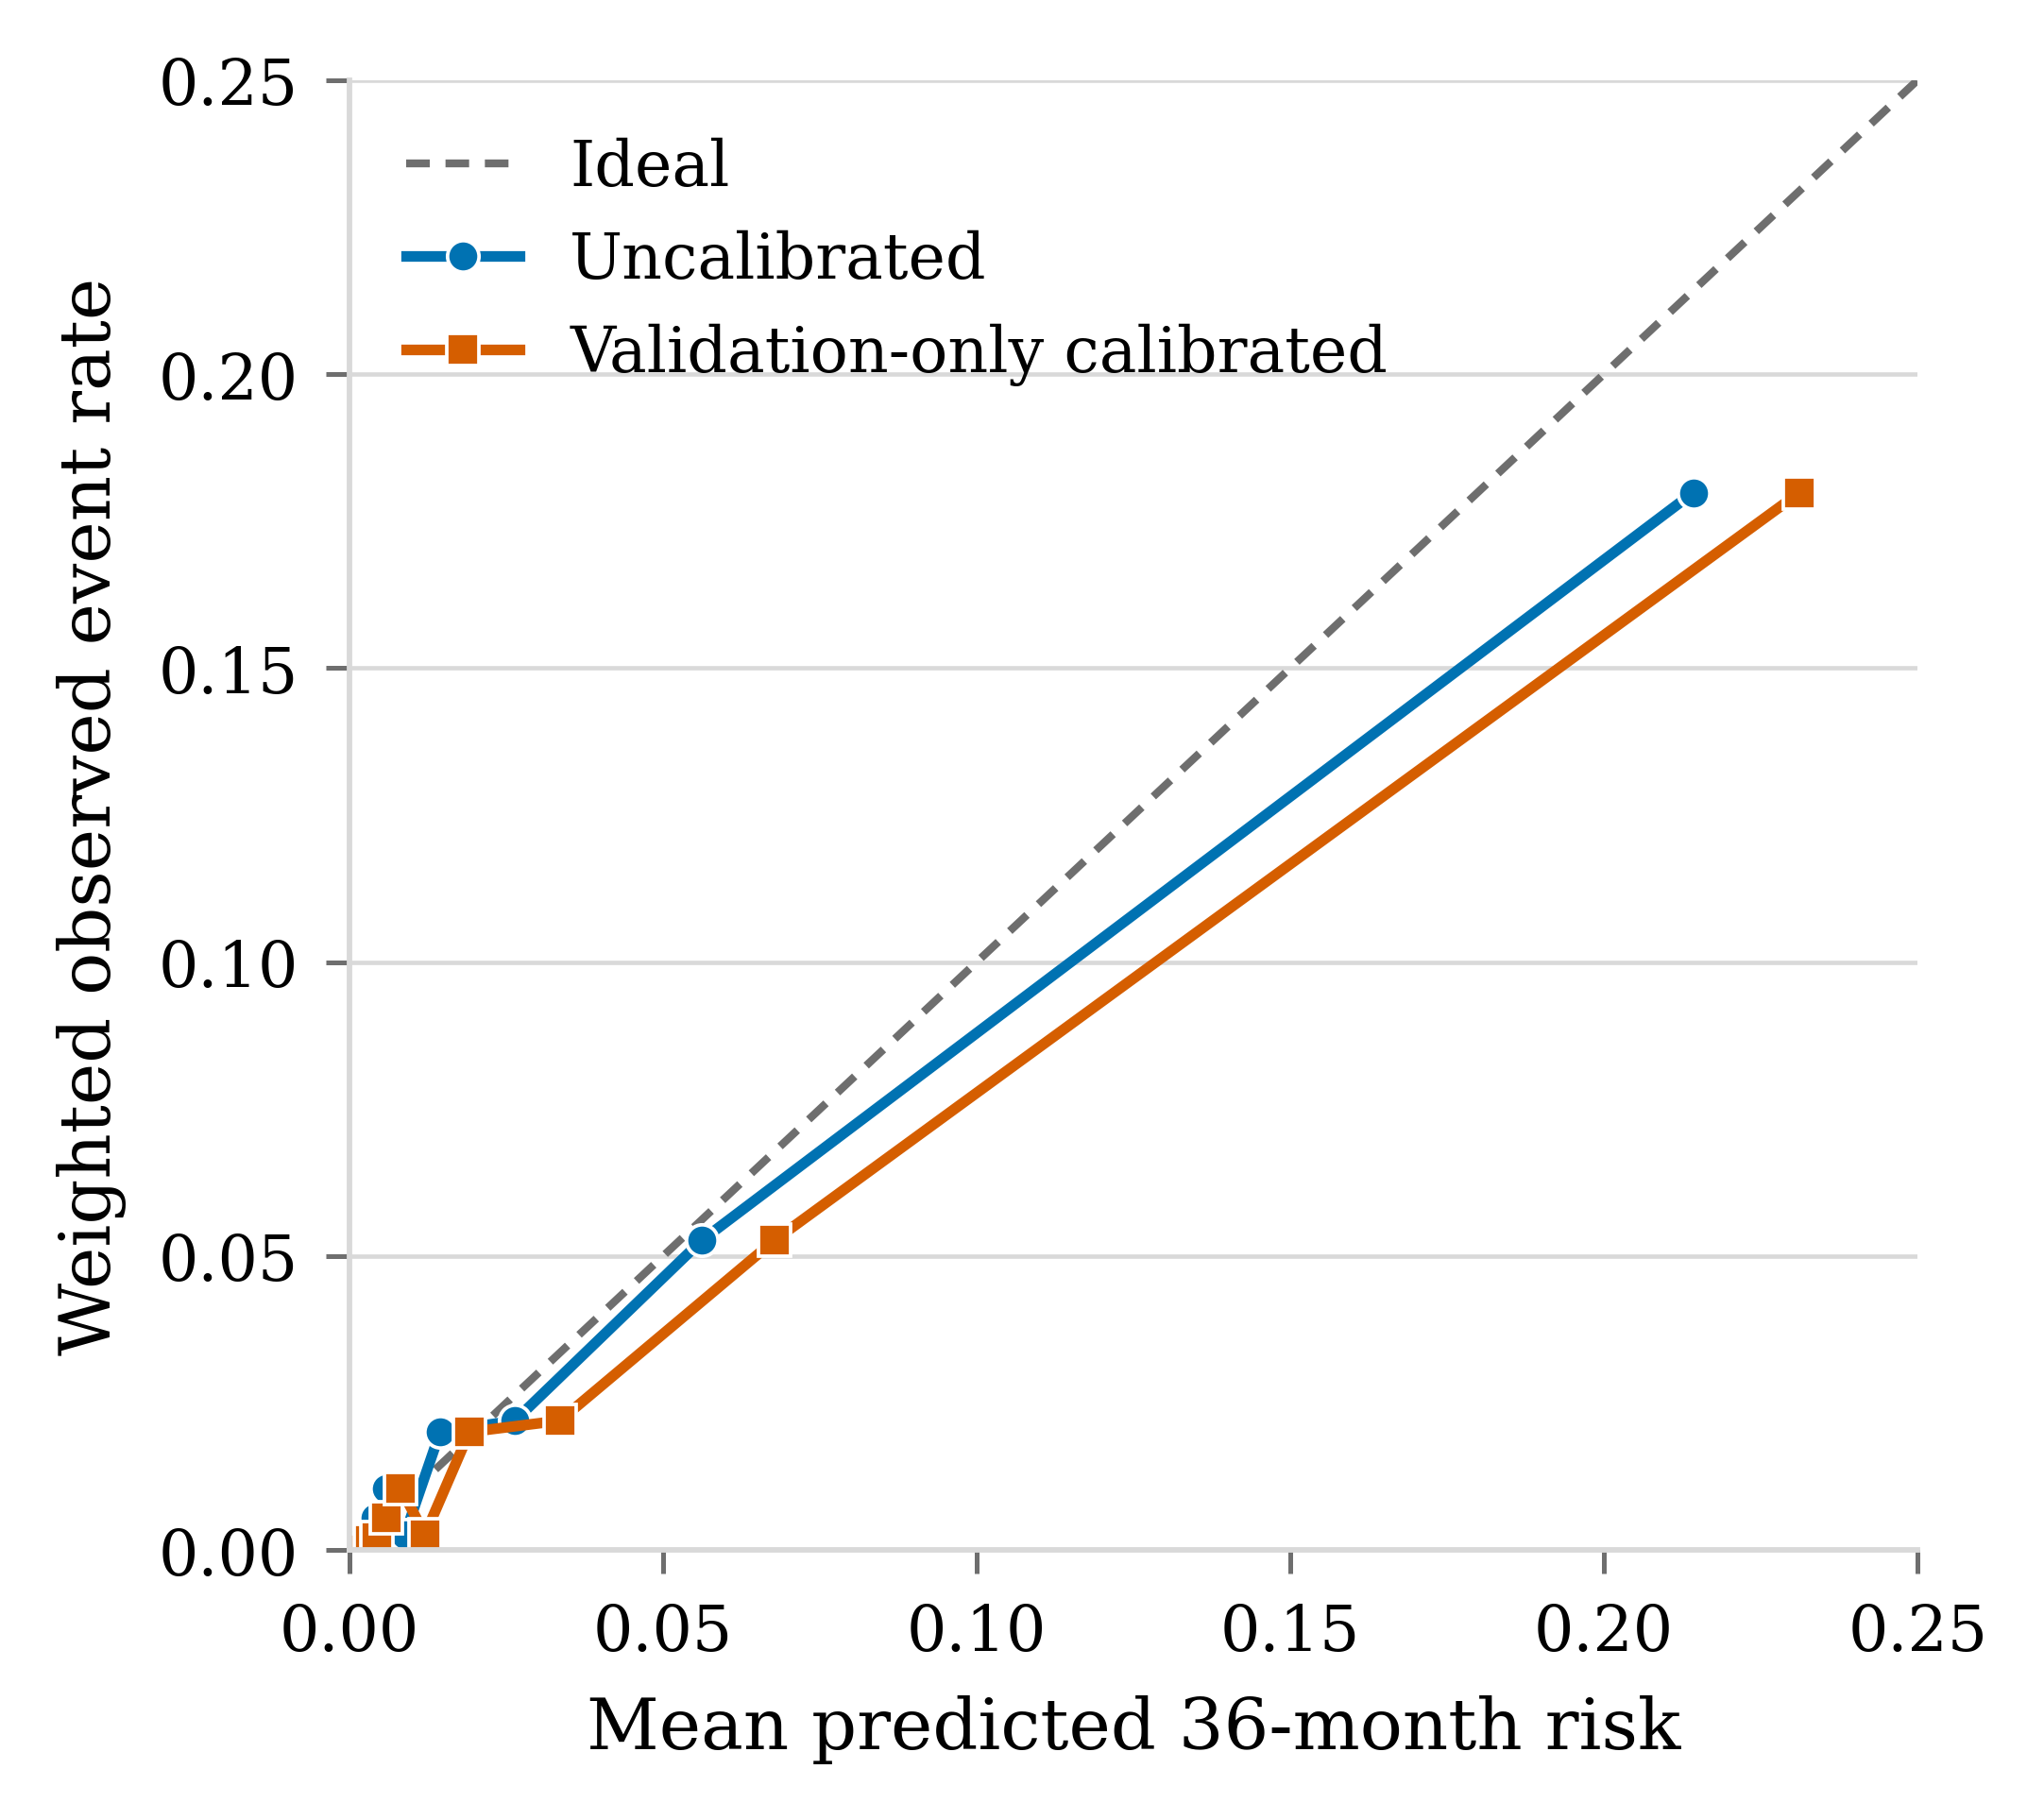
\includegraphics[width=0.72\linewidth]{primary_calibration.png}
\caption{Weighted calibration of the frozen CARE-State predictions on the NHANES 2015--2016 36-month test. Points represent prediction deciles, with mean predicted risk on the horizontal axis and weighted observed event rate on the vertical axis; the two-parameter adapter was fitted on NHANES 2013--2014 only.}
\label{fig:calibration}
\end{figure}

\subsection{Temporal and cross-source transport}
The frozen NHANES 2017--2018 check tested the state after a later survey period and a shorter, prespecified 24-month horizon. CARE-State produced AUROCs of 0.8293, 0.8319, and 0.8324 across the three seeds (mean 0.8312), compared with 0.8195 for GBM and 0.7493 for Cox before calibration. Validation-only calibration changed the Cox AUROC to 0.7514, confirming that the adapter did not alter discrimination. CARE-State was 0.0127 AUROC points above GBM by point estimate, but the paired participant bootstrap 95\% confidence interval, $[-0.0080,0.0358]$, included zero. The evidence is therefore stronger for preservation of ranking than for a statistically established advantage over GBM. The three risk strata remained ordered at 0.0038, 0.0141, and 0.0876. Relative to the primary NHANES test, the high-risk event rate decreased from 0.104 to 0.0876 and the low-risk rate increased from 0.002 to 0.0038, while the ordering was retained. The model thus preserved relative risk structure despite a shift in the absolute event scale.

The NHIS analysis introduced a survey-source change in addition to temporal change and restricted the feature map to the prespecified self-report/BMI intersection. After fitting the two-parameter adapter on NHIS 2016, CARE-State achieved AUROCs of 0.8468, 0.8507, and 0.8476 on NHIS 2017 (mean 0.8484). The adapted risk strata were 0.002, 0.009, and 0.055, corresponding to an approximately 27.5-fold difference between the high- and low-risk groups. Across seeds, the paired bootstrap changes in Brier score were -0.0102, -0.0055, and -0.0048, with every reported 95\% interval below zero. Direct NHANES calibration preserved discrimination but yielded Brier scores of approximately 0.0221--0.0277, compared with 0.0173--0.0175 after NHIS calibration. This separation between stable AUROC and lower Brier error identifies two distinct transport properties: the frozen state carries the participant ordering into the new survey source, while the source-specific adapter adjusts the absolute-risk scale to the target event distribution and measurement context. The result is a survey-source transport test under a reduced feature intersection, not validation of the full laboratory-rich feature map.

Together, the two transport blocks show a consistent pattern across distinct shifts. The state preserved a low-to-high risk ordering in both the later NHANES period and the reduced-feature NHIS source, while the absolute event levels changed with cohort and horizon. Figure~\ref{fig:strata} displays this pattern directly, and Tables~\ref{tab:strata} and~\ref{tab:transport} provide the corresponding event rates and seed-level transport estimates.

\begin{figure}[t!]
\centering
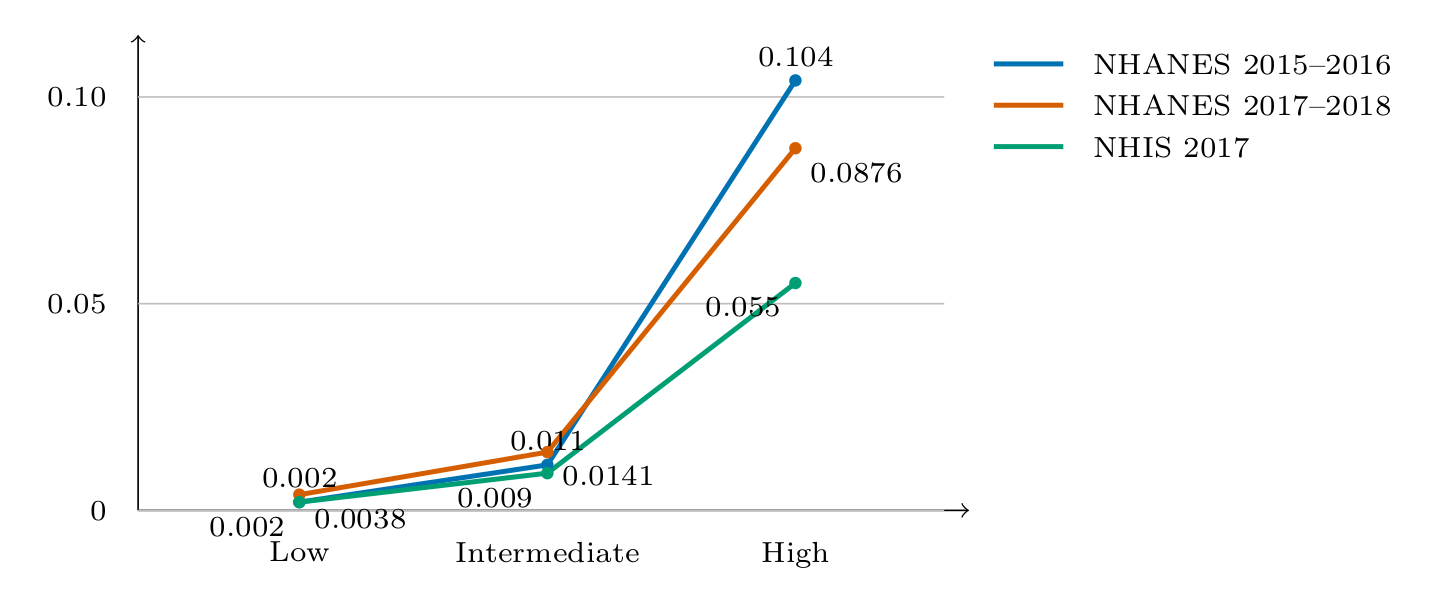
\includegraphics[width=\linewidth]{strata.png}
\caption{Weighted event rates by CARE-State risk stratum. The three lines correspond to the primary NHANES temporal test, the frozen NHANES 2017--2018 check, and the NHIS 2017 survey-source transport test after calibration on NHIS 2016. The curves show risk ordering and cohort-level shifts in absolute event rates.}
\label{fig:strata}
\end{figure}

The corresponding aggregate event rates are listed in Table~\ref{tab:strata}. This table makes the preserved low-to-high ordering explicit while keeping the cohort-specific shifts visible.

\begin{table}[t]
\centering
\caption{CARE-State risk-stratum event rates across the tested cohorts.}
\label{tab:strata}
\small
\begin{tabularx}{0.98\linewidth}{>{\raggedright\arraybackslash}X c c c r}
\toprule
Evaluation block & Low risk & Intermediate risk & High risk & Participants / events \\
\midrule
NHANES 2015--2016, 36 months & 0.0020 & 0.0110 & 0.1040 & 5,710 / 186 \\
NHANES 2017--2018, 24 months & 0.0038 & 0.0141 & 0.0876 & 2,910 / 110 \\
NHIS 2017, 24 months after NHIS 2016 calibration & 0.0020 & 0.0090 & 0.0550 & 26,267 / 656 \\
\bottomrule
\end{tabularx}
\end{table}

\begin{table}[t]
\centering
\caption{Frozen temporal and cross-source transport results. AUROC values are shown for each training seed.}
\label{tab:transport}
\begin{tabular}{p{0.38\linewidth}p{0.24\linewidth}p{0.27\linewidth}}
\toprule
Evaluation & CARE-State & Reference / uncertainty \\
\midrule
NHANES 2017--2018, 24 months & 0.8293, 0.8319, 0.8324 & GBM 0.8195; paired AUROC CI vs GBM $[-0.0080,0.0358]$ \\
NHIS 2017, 24 months after NHIS 2016 calibration & 0.8468, 0.8507, 0.8476 & Brier changes -0.0102, -0.0055, -0.0048; all CIs below zero \\
\bottomrule
\end{tabular}
\end{table}

The two transport blocks should therefore be read as complementary rather than interchangeable tests. The temporal check primarily supports stability of ranking under time shift, whereas the NHIS block additionally tests whether the absolute-risk scale can be recovered after a source change through a prespecified adapter. In both settings, low-to-high risk ordering was retained even though the absolute event levels changed with cohort, source, and prediction horizon. Figure~\ref{fig:strata} displays this common ordering pattern, and Tables~\ref{tab:strata} and \ref{tab:transport} provide the corresponding event rates and seed-level transport estimates.

\subsection{Domain-specific response to missingness}
The masking experiments separated the domains that support ranking from those that support absolute-risk estimation. Relative to the complete-input primary test, cardiovascular masking produced an AUROC of 0.8757 (SD 0.0016), metabolic masking 0.8731 (SD 0.0011), and renal masking 0.8553 (SD 0.0012). These correspond to AUROC changes of +0.0038, +0.0012, and -0.0166, respectively, from the complete CARE-State value of 0.8719. The largest discrimination change followed demographic masking: AUROC fell to 0.7037 (SD 0.0091), a decrease of 0.1682 points. By comparison, renal masking produced a much smaller AUROC decrease but the largest increase in probability error. Its Brier score rose to 0.0252, compared with 0.0208 for complete input.

The Brier results confirmed that the sensitivity pattern was not a simple ordering of domains by overall importance. Cardiovascular masking yielded a Brier score of 0.0209, demographic masking 0.0224, metabolic masking 0.0228, and renal masking 0.0252. Relative to complete input, these were increases of 0.0001, 0.0016, 0.0020, and 0.0044, respectively. Cardiovascular and metabolic masking therefore left ranking near the complete-input estimate, but their effects on probability error were not identical; renal masking affected calibration more strongly than discrimination, whereas demographic masking affected discrimination most strongly. The small positive AUROC changes under cardiovascular and metabolic masking should be read as stability under this particular perturbation, not as evidence that withholding information improves prediction. Figure~\ref{fig:masking} and Table~\ref{tab:masking} summarize the separation between discrimination sensitivity and calibration sensitivity.

\begin{figure}[t!]
\centering
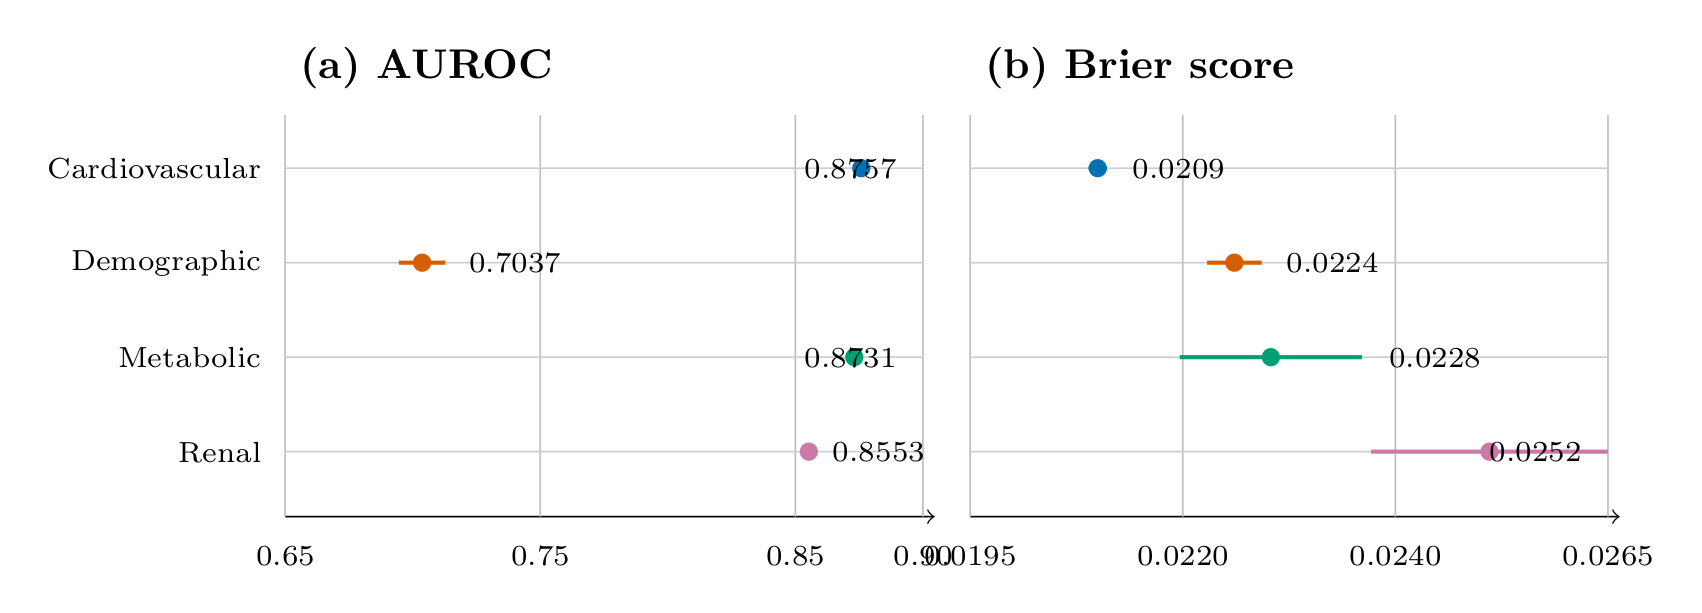
\includegraphics[width=\linewidth]{masking.png}
\caption{Domain-specific response to masking on the NHANES 2015--2016 test cohort. Points show means and horizontal whiskers show standard deviations for cardiovascular, demographic, metabolic, and renal masking. The narrowed x-axis ranges resolve between-domain differences; exact values are given in Table~\ref{tab:masking}.}
\label{fig:masking}
\end{figure}

\begin{table}[t]
\centering
\caption{Domain-specific masking results on the NHANES 2015--2016 test cohort.}
\label{tab:masking}
\begin{tabular}{lcc}
\toprule
Masked domain & Weighted AUROC (mean $\pm$ SD) & Brier score (mean $\pm$ SD) \\
\midrule
Cardiovascular & 0.8757 $\pm$ 0.0016 & 0.0209 $\pm$ 0.0001 \\
Demographic & 0.7037 $\pm$ 0.0091 & 0.0224 $\pm$ 0.0003 \\
Metabolic & 0.8731 $\pm$ 0.0011 & 0.0228 $\pm$ 0.0010 \\
Renal & 0.8553 $\pm$ 0.0012 & 0.0252 $\pm$ 0.0013 \\
\bottomrule
\end{tabular}
\end{table}

\subsection{State-level interpretability and failure modes}
The results define two complementary, directly observable properties of the CARE-State output. First, the shared state produces three risk strata with ordered event rates, and that ordering persists across the primary NHANES test, the later NHANES period, and the independent NHIS source (Figure~\ref{fig:strata}, Table~\ref{tab:strata}). Second, the masking analysis assigns different failure modes to different clinical domains: demographic evidence is most important for maintaining discrimination, while renal evidence is most important for maintaining probability accuracy (Figure~\ref{fig:masking}, Table~\ref{tab:masking}). The model is therefore interpretable in an operational sense: the risk state can be examined through its population stratification, its response to cohort shift, and the performance dimension that deteriorates when a domain is unavailable. This is more specific than describing the model as simply ``robust to missingness''; the experiments show which aspect of prediction remains stable and which aspect becomes unreliable under each domain-level perturbation.

\section{Discussion}
This study did not ask which algorithm achieves the highest score on a single data split. It asked whether a population risk state can preserve the same ordering semantics when survey period, survey source, and available health evidence change together. In the primary NHANES test, CARE-State achieved a weighted AUROC of 0.8719 versus 0.8671 for weighted gradient boosting; the corresponding Brier scores were 0.0208 and 0.0207, showing that discrimination and probability error did not move in the same direction. Across the later NHANES period and the NHIS survey-source transport test, the most stable evidence was not a numerical lead on one metric, but the persistence of ordered low-, intermediate-, and high-risk strata. CARE-State is therefore best understood as an auditable population-surveillance framework that jointly represents risk ordering, absolute probability, and evidence-availability failure behavior, rather than as a claim of universal superiority over every reference model.

The methodological meaning of CARE-State begins with an explicit separation between a measurement and the availability of that measurement. In public surveys, missingness can reflect subsample selection, nonresponse, assay availability, or changes in the survey instrument; it is not equivalent to a normal value. If missing values are imputed and passed to a single predictor, the model cannot reliably distinguish a low observed value from evidence that was never collected. CARE-State combines each domain measurement vector with an availability mask, so the state records both what health evidence is present and whether that evidence was observable under the current survey process. Missingness is consequently part of the state semantics rather than a purely numerical preprocessing decision. This distinction separates the proposed representation from missing-data methods whose primary objective is value reconstruction or sequence completion.

The domain-masking results show that health evidence does not have a single, interchangeable notion of importance. Masking the demographic domain reduced AUROC from 0.8719 to 0.7037, indicating that demographic evidence primarily supports ranking across population groups. Masking the renal domain reduced AUROC to 0.8553 but increased the Brier score to 0.0252, identifying renal evidence as the principal support for probability-scale accuracy. Discrimination and calibration therefore depend on different evidence pathways: demographic information helps determine who occupies a higher-risk position, whereas renal information helps map that position to a credible event probability. This moves interpretation beyond a generic variable-importance ranking toward a functional account of what each domain contributes to the prediction system. The operational implication is limited to evidence-audit prioritization in a survey pipeline; it is not a clinical recommendation.

The temporal and source analyses support treating transport as two separately managed problems. The frozen state carries relative risk ordering, while the calibration adapter adjusts the source-specific probability scale. In NHANES 2017--2018, the mean AUROC across the three training seeds was 0.8312, and the strata remained ordered at event rates of 0.0038, 0.0141, and 0.0876. In the NHIS transfer analysis, AUROC remained between 0.8468 and 0.8507, while an adapter estimated only on the calibration cohort reduced Brier error. This pattern indicates that cross-source application should not be reduced to retraining a larger predictor: when the ordering remains informative, the first task is to test and recalibrate the probability scale without replacing the learned state. The result is consistent with the established distinction between discrimination and calibration \cite{steyerberg_2010_prediction,van_calster_2019_calibration}, and allows external validation to answer two separate questions: whether ranking transports and whether probabilities require recalibration.

The study is consequently positioned beyond a conventional benchmark. Cox regression and gradient boosting provide contextual reference points and establish whether the proposed state sacrifices basic predictive performance. The primary object of evaluation, however, is whether an interpretable state can retain its meaning under prespecified temporal and survey-source changes. Risk-stratum event rates, frozen transport, validation-only calibration, and domain masking are evaluated together rather than collapsing the contribution into a single AUROC leaderboard. Research on distribution shift shows that in-domain ranking does not reliably predict out-of-domain probability quality, and that probability degradation can occur while ranking remains relatively stable \cite{koh_2021_wilds,ovadia_2019_uncertainty}. CARE-State addresses this evaluation gap by treating ``can still rank'' and ``can still assign credible probabilities'' as distinct output properties that require separate evidence.

For public-health use, the three risk states provide a survey-population summary rather than an individual diagnosis. A digital-health surveillance pipeline could compare the weighted composition of risk strata across survey cycles, flag a change in calibration after a source transition, and use the masking audit to prioritize data-quality checks or evidence acquisition. Survey-weighted event rates connect the output to the target population represented by the sampling design, making comparisons across survey cycles interpretable at the population level. The masking audit yields conditional evidence-audit rules: when demographic evidence is unavailable, the primary concern is weakened risk ordering; when renal evidence is unavailable, the primary concern is probability recalibration. The framework is therefore suited to population surveillance and survey-design assessment under constrained measurement capacity. It does not convert an observational risk score into a treatment recommendation or an intervention effect.

The credibility of the evidence is strengthened by prespecified validation boundaries. The primary test was held out chronologically, the later NHANES period and final NHIS test set were evaluated after model freezing, and the NHIS 2016 calibration cohort was separated from the NHIS 2017 test cohort. Survey weights were used throughout the main comparisons and risk-stratum analyses. Three independent seeds and paired bootstrap contrasts expose estimation variability; notably, the paired 95\% confidence interval for the later-NHANES AUROC difference between CARE-State and GBM was $[-0.0080,0.0358]$. This supports competitive discrimination and stable risk ordering, while it does not justify presenting the point estimate as established model superiority. The reporting therefore keeps the strength of the methodological claim aligned with the strength of the statistical evidence.

The scope of the conclusions is defined by the data sources and validation design. The analysis uses public surveys and mortality linkage files, supporting associative prediction and transport analysis within the tested populations rather than causal effect estimation. The temporal and source analyses use different follow-up horizons, and the NHIS transfer uses a self-report/BMI feature intersection rather than the complete laboratory-rich NHANES map; the transport claim consequently applies to the specified shared feature boundary. The aggregate local package does not include the server-side retraining pipeline, so the implementation should not be represented as a fully self-contained software release. Further work should evaluate additional survey releases, prespecified subgroup calibration, probability stability across outcome windows, and interpretation and decision impact in a governed population-health workflow. These tests directly assess whether the semantics of CARE-State persist beyond the public datasets used here, rather than merely adding more random seeds.

\section{Conclusions}
CARE-State organizes population-health evidence, evidence availability, risk ordering, and probability calibration into a missingness-aware risk state for public-health surveys. The experiments show that the state preserves ordered risk strata across the tested temporal and survey-source changes, maintains competitive probability performance after calibration on an independent survey source, and exposes distinct roles for demographic and renal evidence through controlled domain masking. Its contribution is not a higher score on a single benchmark; it is a bounded population-surveillance representation that makes transport behavior and evidence-audit failure boundaries observable.

Within the current data and validation boundaries, CARE-State is supported as an auditable population-risk analysis framework for comparing survey periods, identifying ordered risk strata, and prioritizing evidence-quality checks. Broader use requires validation on additional survey releases, prespecified subgroup calibration, a complete retraining implementation, and evaluation of interpretation and decision impact under population-health governance.

\authorcontributions{Conceptualization, Zhi Jin and Shuang Wu; methodology, Zhi Jin, Hua Sun, Quanwei Sheng, and Shuang Wu; software, Zhi Jin and Quanwei Sheng; validation, Hua Sun and Shuang Wu; formal analysis, Zhi Jin and Hua Sun; investigation and data curation, Quanwei Sheng; writing---original draft preparation, Zhi Jin; writing---review and editing, Hua Sun, Quanwei Sheng, and Shuang Wu; visualization, Zhi Jin; supervision, Shuang Wu. All authors have read and agreed to the published version of the manuscript.}
\funding{This research received no external funding.}
\institutionalreview{Ethical review and approval were not required because this study used de-identified, publicly available secondary data and involved no new participant contact or intervention.}
\informedconsent{Not applicable because the study used de-identified, publicly available secondary data and involved no direct participant contact.}
\dataavailability{All datasets analyzed in this study are publicly available from the U.S. National Center for Health Statistics. NHANES source-data directories used for the chronological analysis were: 2007--2008, \url{https://wwwn.cdc.gov/Nchs/Data/Nhanes/Public/2007/DataFiles/}; 2009--2010, \url{https://wwwn.cdc.gov/Nchs/Data/Nhanes/Public/2009/DataFiles/}; 2011--2012, \url{https://wwwn.cdc.gov/Nchs/Data/Nhanes/Public/2011/DataFiles/}; 2013--2014, \url{https://wwwn.cdc.gov/Nchs/Data/Nhanes/Public/2013/DataFiles/}; 2015--2016, \url{https://wwwn.cdc.gov/Nchs/Data/Nhanes/Public/2015/DataFiles/}; and 2017--2018, \url{https://wwwn.cdc.gov/Nchs/Data/Nhanes/Public/2017/DataFiles/}. The corresponding NHANES public-use mortality files were 2007--2008, \url{https://ftp.cdc.gov/pub/Health_Statistics/NCHS/datalinkage/linked_mortality/NHANES_2007_2008_MORT_2019_PUBLIC.dat}; 2009--2010, \url{https://ftp.cdc.gov/pub/Health_Statistics/NCHS/datalinkage/linked_mortality/NHANES_2009_2010_MORT_2019_PUBLIC.dat}; 2011--2012, \url{https://ftp.cdc.gov/pub/Health_Statistics/NCHS/datalinkage/linked_mortality/NHANES_2011_2012_MORT_2019_PUBLIC.dat}; 2013--2014, \url{https://ftp.cdc.gov/pub/Health_Statistics/NCHS/datalinkage/linked_mortality/NHANES_2013_2014_MORT_2019_PUBLIC.dat}; 2015--2016, \url{https://ftp.cdc.gov/pub/Health_Statistics/NCHS/datalinkage/linked_mortality/NHANES_2015_2016_MORT_2019_PUBLIC.dat}; and 2017--2018, \url{https://ftp.cdc.gov/pub/Health_Statistics/NCHS/datalinkage/linked_mortality/NHANES_2017_2018_MORT_2019_PUBLIC.dat}. The NHIS source files used for the independent-source analysis were the 2016 adult file, \url{https://ftp.cdc.gov/pub/Health_Statistics/NCHS/Datasets/NHIS/2016/samadultcsv.zip}, and person file, \url{https://ftp.cdc.gov/pub/Health_Statistics/NCHS/Datasets/NHIS/2016/personsxcsv.zip}; and the corresponding 2017 adult file, \url{https://ftp.cdc.gov/pub/Health_Statistics/NCHS/Datasets/NHIS/2017/samadultcsv.zip}, and person file, \url{https://ftp.cdc.gov/pub/Health_Statistics/NCHS/Datasets/NHIS/2017/personsxcsv.zip}. The corresponding NHIS public-use mortality files were 2016, \url{https://ftp.cdc.gov/pub/Health_Statistics/NCHS/datalinkage/linked_mortality/NHIS_2016_MORT_2019_PUBLIC.dat}, and 2017, \url{https://ftp.cdc.gov/pub/Health_Statistics/NCHS/datalinkage/linked_mortality/NHIS_2017_MORT_2019_PUBLIC.dat}. All files are de-identified public-use records; no private or restricted patient-level data were used.}
\codeavailability{The repository at \url{https://github.com/Hajimi-Sudo/care-state-survey-risk} contains the aggregate derived results, figure-generation scripts, manuscript sources, and documentation needed to reproduce the reported aggregate figures. It does not contain individual-level NHANES or NHIS records or the original server-side retraining pipeline. The public-use source files should be obtained from the links provided in the Data Availability Statement.}
\conflictsofinterest{The authors declare that there is no conflict of interest.}

\section*{References}
\bibliographystyle{plainnat}
\bibliography{refs}
\end{document}
